\documentclass[a4paper]{article} 
\usepackage{amsmath,amsfonts,bm}
\usepackage{hyperref}
\usepackage{amsthm} 
\usepackage{geometry}
\usepackage{amssymb}
\usepackage{pstricks-add}
\usepackage{framed,mdframed}
\usepackage{graphicx,color} 
\usepackage{mathrsfs,xcolor} 
\usepackage[all]{xy}
\usepackage{fancybox} 
\usepackage{xeCJK}
\newtheorem*{theorem}{定理}
\newtheorem*{lemma}{引理}
\newtheorem*{corollary}{推论}
\newtheorem*{exercise}{习题}
\newtheorem*{example}{例}
\geometry{left=2.5cm,right=2.5cm,top=2.5cm,bottom=2.5cm}
\setCJKmainfont[BoldFont=Adobe Fangsong Std]{Adobe Fangsong Std}
\renewcommand{\today}{\number\year 年 \number\month 月 \number\day 日}
\newcommand{\D}{\displaystyle}\newcommand{\ri}{\Rightarrow}
\newcommand{\ds}{\displaystyle} \renewcommand{\ni}{\noindent}
\newcommand{\pa}{\partial} \newcommand{\Om}{\Omega}
\newcommand{\om}{\omega} \newcommand{\sik}{\sum_{i=1}^k}
\newcommand{\vov}{\Vert\omega\Vert} \newcommand{\Umy}{U_{\mu_i,y^i}}
\newcommand{\lamns}{\lambda_n^{^{\scriptstyle\sigma}}}
\newcommand{\chiomn}{\chi_{_{\Omega_n}}}
\newcommand{\ullim}{\underline{\lim}} \newcommand{\bsy}{\boldsymbol}
\newcommand{\mvb}{\mathversion{bold}} \newcommand{\la}{\lambda}
\newcommand{\La}{\Lambda} \newcommand{\va}{\varepsilon}
\newcommand{\be}{\beta} \newcommand{\al}{\alpha}
\newcommand{\dis}{\displaystyle} \newcommand{\R}{{\mathbb R}}
\newcommand{\N}{{\mathbb N}} \newcommand{\cF}{{\mathcal F}}
\newcommand{\gB}{{\mathfrak B}} \newcommand{\eps}{\epsilon}
\renewcommand\refname{参考文献}
\begin{document}
\title{\bf{从《复分析——可视化方法》习题2.9.7到最大模原理}} \author{\small{叶卢
    庆\footnote{叶卢庆(1992---),男,杭州师范大学理学院数学与应用数学专业
      本科在读,E-mail:h5411167@gmail.com}}\\{\small{杭州师范大学理学院,数学112,学号:1002011005}}}
\maketitle
\begin{enumerate}
\item画出 $C(z)=(z+1)(z-1)(z+1+i)$ 的模曲面的草图.由此画出卡西尼曲线
$|C(z)|=const.$ 的草图.
\begin{proof}[\bf{解}]
模曲面草图如下:\\
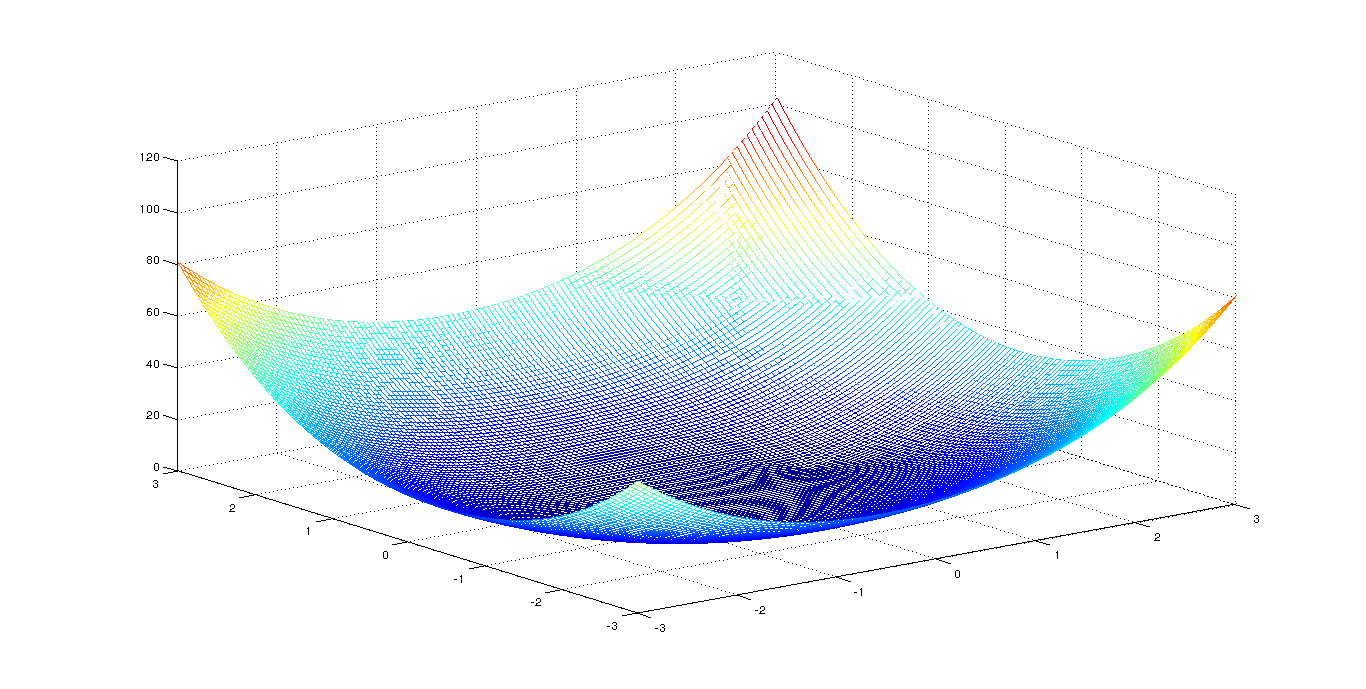
\includegraphics[width=0.8\textwidth]{/home/luqing/math/visual-complex-analysis/exercise2-9-7.png}

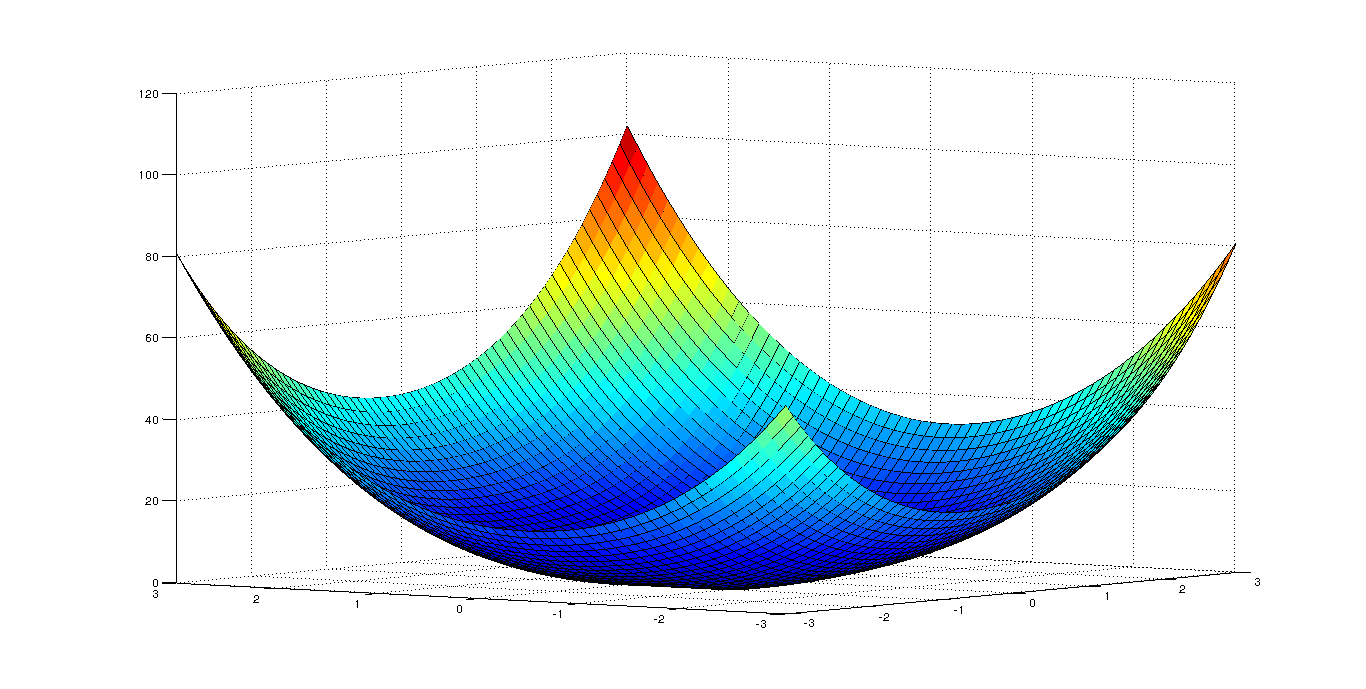
\includegraphics[width=0.8\textwidth]{/home/luqing/math/visual-complex-analysis/exercise2-9-7-1.png}

等高线如下.这也是以 $-1,1,-1-i$ 为焦点的卡西尼曲线族的样子.

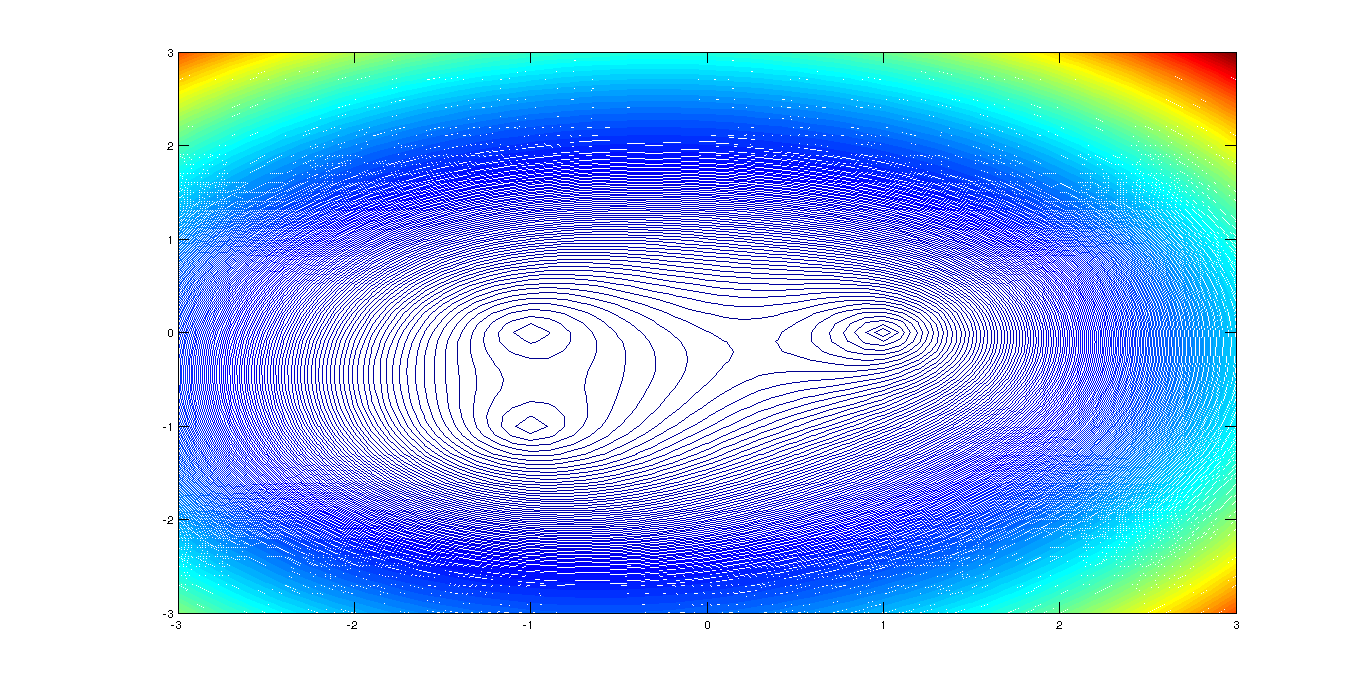
\includegraphics[width=0.8\textwidth]{/home/luqing/math/visual-complex-analysis/exercise2-9-7-3.png}
\end{proof}
\item 刚才画出的卡西尼曲线的正交轨道的意义是什么?
  \begin{proof}[\bf{解}]
模曲面的高度沿着平面上某一条曲线变化速率最快,那条曲线就是卡西尼曲线的正交轨
道.
  \end{proof}
\item $|C(z)|$ 有无局部极大或非零的局部极小?
  \begin{proof}[\bf{解}]
    无.因为观察发现每条卡西尼曲线都是连续的.而卡西尼曲线是模曲面的等高
    线.在这种情况下,$|C(z)|$ 的局部极大和非零的局部极小是不可能存在的.
  \end{proof}
\item 若 $D$ 是一圆盘(甚至是比较任意的形状),$|C(z)|$ 在 $D$ 上的最大值
  可否发生在 $D$ 的内点或者只能发生在 $D$ 的边界点上?最小值又如何?
  \begin{proof}[\bf{解}]
    无论是最大值还是最小值,都只可能发生在$D$ 的边界点,而不可能出现在
    $D$ 的内点.这也是由卡西尼曲线的连续性决定的,而卡西尼曲线是模等高线.
  \end{proof}
\item 若用任意多项式代替 $C(z)$,对这些问题是否有同样的答案.对于仅仅知
  道可以表示为一幂级数的函数又如何.
  \begin{proof}[\bf{解}]
都有一样的答案.下面我们来具体阐述.设 $P(z)$ 是最高次项系数为 $1$ 的 $n$ 次多项式,则根据分解
定理,易得 $P$可以分解为
$$
P(z)=(z-a_1)(z-a_2)\cdots (z-a_m),
$$
则 
$$
|P(z)|=|z-a_1||z-a_2|\cdots |z-a_m|.
$$
设 $|P(z)|=k$,其中 $k>0$,则
\begin{equation}\label{eq:6}
|z-a_1||z-a_2|\cdots |z-a_m|=k
\end{equation}
是有 $m$ 个焦点的卡西尼曲线,$m$ 个焦点分别为 $a_1,a_2,\cdots,a_m$.下面
证明有 $m$ 个焦点的卡西尼曲线是连续的曲线.把复平面转化为直角坐标平面,
复数 $z$ 为 $(x,y)$,$a_i$ 为 $(a_{ix},a_{iy})$,其中
$x,y,a_{ix},a_{iy}\in \mathbf{R}$.则方程 \eqref{eq:6} 变为
\begin{equation}
  \label{eq:7}
  [(x-a_{1x})^2+(y-a_{1y})^2]\times \cdots\times [(x-a_{mx})^2+(y-a_{my})^2]=k^2.
\end{equation}
令 $f(x,y)=  [(x-a_{1x})^2+(y-a_{1y})^2]\times \cdots\times
[(x-a_{mx})^2+(y-a_{my})^2]-k^2$,则
$$
\frac{\pa f}{\pa x}=\sum_{i=1}^{m} 2(x-a_{ix})\frac{f(x,y)+k^2}{(x-a_{ix})^2+(y-a_{iy})^2},
$$
$$
\frac{\pa f}{\pa y}=\sum_{i=1}^m 2(y-a_{iy})\frac{f(x,y)+k^2}{(x-a_{ix})^2+(y-a_{iy})^2}.
$$
下面我们来证明, $\frac{\pa f}{\pa x},\frac{\pa f}{\pa y}$ 一般来说,不
会都为$0$,即使都为 $0$ 了,也只是发生在孤立点上.\\

我们先来看 $n=2$ 的简单情形.此时,
$$
\frac{\pa f}{\pa x}=2(x-a_{1x})[(x-a_{2x})^2+(y-a_{2y})^2]+2(x-a_{2x})[(x-a_{1x})^2+(y-a_{1y})^2],
$$
$$
\frac{\pa f}{\pa y}=2(y-a_{1y})[(x-a_{2x})^2+(y-a_{2y})^2]+2(y-a_{2y})[(x-a_{1x})^2+(y-a_{1y})^2].
$$
如果 $\frac{\pa f}{\pa x}$ 和 $\frac{\pa f}{\pa y}$ 都为 $0$,则
$$
(x-a_{1x})(y-a_{2y})-(y-a_{1y})(x-a_{2x})=0.
$$
于是,
$$
\begin{vmatrix}
  x-a_{1x}&y-a_{1y}\\
x-a_{2x}&y-a_{2y}
\end{vmatrix}=0.
$$
由此可得向量 $(x-a_{1x},y-a_{1y})$ 和向量 $(x-a_{2x},y-a_{2y})$ 线性相
关且长度相等,且这两个向量不同.因此
$$
(x-a_{1x},y-a_{1y})=-(x-a_{2x},y-a_{2y}).
$$
解得
$$
x=\frac{a_{1x}+a_{2x}}{2},y=\frac{a_{1y}+a_{2y}}{2}.
$$
这种情况只可能在卡西尼曲线变成Bernoulli双纽线的情形发生,此时 $(x,y)$
变为双纽线的自交点.\\

我们现在再来看 $n=3$ 的情形.此时,
\begin{align*}
\frac{\pa f}{\pa x}&=2(x-a_{1x})[(x-a_{2x})^2+(y-a_{2y})^2][(x-a_{3x})^2+(y-a_{3y})^{2}]+2(x-a_{2x})[(x-a_{1x})^2+(y-a_{1y})^2][(x-a_{3x})^2\\&+(y-a_{3y})^{2}]+2(x-a_{3x})[(x-a_{1x})^2+(y-a_{1y})^2][(x-a_{2x})^2+(y-a_{2y})^{2}],
\end{align*}
\begin{align*}
  \frac{\pa f}{\pa y}&=2(y-a_{1y})[(x-a_{2x})^2+(y-a_{2y})^2][(x-a_{3x})^2+(y-a_{3y})^{2}]+2(y-a_{2y})[(x-a_{1x})^2+(y-a_{1y})^2][(x-a_{3x})^2\\&+(y-a_{3y})^{2}]+2(y-a_{3y})[(x-a_{1x})^2+(y-a_{1y})^2][(x-a_{2x})^2+(y-a_{2y})^{2}].
\end{align*}
如果 $\frac{\pa f}{\pa x},\frac{\pa f}{\pa y}$ 都为 $0$,则在空间直角坐
标系里,向量 $(x-a_{1x},x-a_{2x},x-a_{3x})$ 和向量
$(y-a_{1y},y-a_{2y},y-a_{3y})$ 都与向量
$([(x-a_{2x})^2+(y-a_{2y})^2][(x-a_{3x})^2+(y-a_{3y})^{2}],[(x-a_{1x})^2+(y-a_{1y})^2][(x-a_{3x})^2+(y-a_{3y})^{2}],[(x-a_{1x})^2+(y-a_{1y})^2][(x-a_{2x})^2+(y-a_{2y})^{2}])$
垂直.
  \end{proof}
\end{enumerate}

\end{document}








